\chapter{Results}
\section{Cumulative apparent fishing hours}

In total, there were 213 unique longliners and purse seiners recorded for 2015-2024. These vessels together accounted
for an average of 5115 fishing days per year, with an average of 24 days per vessel per year. 

\medskip

\begin{figure}[h]
    \subplot{2}
    {width=1\linewidth, trim=1.2cm 0 1.2cm 0,clip}
    {Figures/plots/sum_cv.pdf}
    {%
    Summary statistics for both longliners and purse-seiners. \subref{sub0:fig:sum_cv}) Cumulative fishing hours in the Mediterranean (2015-2024). 
    Colors are on a log-scale. \subref{sub1:fig:sum_cv}) Coefficient of variation between years (standard deviation divided by mean) for each cell.
    }{fig:sum_cv}
\end{figure}

Areas that show  the highest effort throughout
the study time include the Mediterranean coast of Spain, around Sardinia and Sicily, south of Malta, the Adriatic, and
south of Cyprus \figref{sub0:fig:sum_cv}. Areas with high effort generally also show the lowest coefficient of variation \figref{sub1:fig:sum_cv}.
There does not appear to be any fishing activity based on AIS around the African Mediterranean coast.

\FloatBarrier
\section{Hotspot analysis}
There were numerous persistent longline hotspot areas identified throughout the Mediterranean including the southern coast of Spain, south of Sardinia, 
around Sicily and Malta, as well as south of Cyprus \figref{sub0:fig:longline_hotspots}. These hotspots show however, differing trends. Fishing hours
in the south of Malta appear to be increasing throughout, with a similar trend of increase in the Adriatic Sea. Other areas that appear to be consistent
hotspots like the east of Sicily show a decreasing trend \figref{sub1:fig:longline_hotspots}.

\begin{figure}[h]
    \subplot{2}
    {width=1\linewidth, trim=0.85cm 0 1.2cm 0,clip}
    {Figures/plots/dll_hotspot_trend.pdf}
    {%
    Hotspot percentage and trend scores for longliners in the Mediterranean.
    The percentage reflects the years in which a given cell was a hotspot based on the Getis-Ord Gi* statistic.
    The Z-score is derived from the Mann-Kendall statistic.}
    {fig:longline_hotspots}
\end{figure}

Purse seine hotspots appear persistent around the Balearic Islands, in the Adriatic Sea, and along the Calabrian coast in Italy \figref{sub0:fig:seines_hotspots}.
Trends in these areas show a clear increase around Ibiza and in the central Adriatic while areas around the coast in the Adriatic show a decrease \figref{sub1:fig:seines_hotspots}.
The hotspot area along Calabria shows no clear trend.

\begin{figure}[h]
    \subplot{2}
    {width=1\linewidth, trim=0.4cm 0 0.7cm 0,clip}
    {Figures/plots/pss_hotspot_trend.pdf}
    {%
    Hotspot percentage and trend scores for purse seiners in the Mediterranean.
    The percentage reflects the years in which a given cell was a hotspot based on the Getis-Ord Gi* statistic.
    The Z-score is derived from the Mann-Kendall statistic.}
    {fig:seines_hotspots}
\end{figure}

\FloatBarrier
\section{Temporal changes}
Longline fishing hours show a clear seasonal trend where activity is highest in the summer and lowest in the winter \figref{sub0:fig:longlines_ridge}. Some areas show high
effort earlier in the season in spring (for example south of Malta) and others are more persistent later in the season in fall (for instance around Ibiza).
Daily fishing shows a similar seasonal trend, although the intensity varies between years. The highest annual longline fishing hours throughout the study time were recorded for 2022
and the lowest for 2015 \tabref{tab:year_hours}.

\begin{figure}[htp]
    \customsubplot{2}
    {1\linewidth}                           % width
    {0.5cm 0 0.6cm 0}                       % trim
    {Figures/plots/longlines_ridge_seasons.pdf} % file
    {5,92}                                  % (A) position
    {5,40}                                  % (B) position
    {fig:longlines_ridge}
    {%
    Temporal changes in longline fishing hours. \subref{sub0:fig:longlines_ridge}) Spatial differences between seasons. 
    Hours are summed per season and cell. \subref{sub1:fig:longlines_ridge}) Time series of fishing hours, summed per year 
    and day.}
\end{figure}

\begin{table}[h]
\centering
\caption{Annual sum of fishing hours for purse seiners and longliners.}
\medskip
\begin{tabular}{lcc}
\toprule
\textbf{Year} & \multicolumn{2}{c}{\textbf{Fishing hours}} \\
\cmidrule(lr){2-3}
                 & \textbf{Purse seiners} & \textbf{Longliners} \\
\midrule
2015   & 4,193   & 71,846 \\
2016   & 5,313   & 89,136 \\
2017   & 5,901   & 107,345 \\
2018   & 6,128   & 106,130 \\
2019   & 5,931   & 113,261 \\
2020   & 5,636   & 124,927 \\
2021   & 5,706   & 133,361 \\
2022   & 5,675   & 149,059 \\
2023   & 5,085   & 139,068 \\
2024   & 6,661   & 137,406 \\
\bottomrule
\end{tabular}
\label{tab:year_hours}
\end{table}

Purse seine fishing hours show a very pronounced seasonal trend with a peak in spring \figref{fig:seines_ridge}. The core areas of the fishery
during spring are the Balearic Islands, along the coast of Calabria (south-west Italy), and the central Adriatic. In the Adriatic, there appears to be
purse seine activity throughout the whole year \figref{sub0:fig:seines_ridge}. The purse seine season for large-pelagic species is limited to the months
of May and June and is consistent between years \figref{sub1:fig:seines_ridge}. Highest annual fishing hours for purse seiners were recorded in 2024 and the
lowest in 2015 \tabref{tab:year_hours}.

\begin{figure}
    \customsubplot{2}
    {1\linewidth}
    {1.2cm 0 0.9cm 0}                       % trim
    {Figures/plots/purse_seines_ridge_seasons.pdf} % file
    {3,93.5}                                  % (A) position
    {3,42}                                  % (B) position
    {fig:seines_ridge}
    {%
    Temporal changes in purse seine fishing hours. \subref{sub0:fig:seines_ridge}) Spatial differences between seasons. 
    Hours are summed per season and cell. \subref{sub1:fig:seines_ridge}) Time series of fishing hours, summed per year 
    and day.}
\end{figure}

\FloatBarrier
\section{Flag countries}

Vessels were flagged to a total of 10 countries and the majority of vessels analysed were longliners \tabref{tab:countries_vessels}. 
For an overview of fishing hours for each country see Figure~\ref{fig:longline_effort_countries} and~\ref{fig:seine_effort_countries}.
Italy has the highest amount of both purse seiners and longliners in the GFW data.

\medskip

\begin{table}[h]
\centering
\caption{Number of vessels by country and gear type based on GFW data and national registry information. ‘--’ indicates no recorded vessels for that gear.}
\medskip
\begin{tabular}{lcc}
\toprule
\textbf{Country} & \multicolumn{2}{c}{\textbf{Number of vessels}} \\
\cmidrule(lr){2-3}
                 & \textbf{Purse seiners} & \textbf{Longliners} \\
\midrule
Algeria   & 4   & -- \\
Croatia   & 2   & -- \\
Cyprus    & --  & 25 \\
France    & 14  & -- \\
Greece    & --  & 9 \\
Italy     & 16  & 79 \\
Malta     & --  & 21 \\
Morocco   & 1   & -- \\
Spain     & 5   & 35 \\
Tunisia   & 2   & -- \\
\midrule
\textbf{Total}   & \textbf{44} & \textbf{169} \\
\bottomrule
\end{tabular}
\label{tab:countries_vessels}
\end{table}

Most regions with high fishing activity also have vessels flagged to multiple countries fishing in the same area. Regions with high overlap between flag countries
for longliners include the Balearic Islands, south of Crete, and south of Malta \figref{fig:no_countries}, which are also areas with high fishing hours \figref{sub0:fig:sum_cv}.
For purse seiners, fishing generally is more concentrated and thus, overlap is also higher, as seen in the core fishing areas of the Balearic Islands and south of Malta \figref{fig:no_countries}.

\begin{figure}[H]
    \centering
    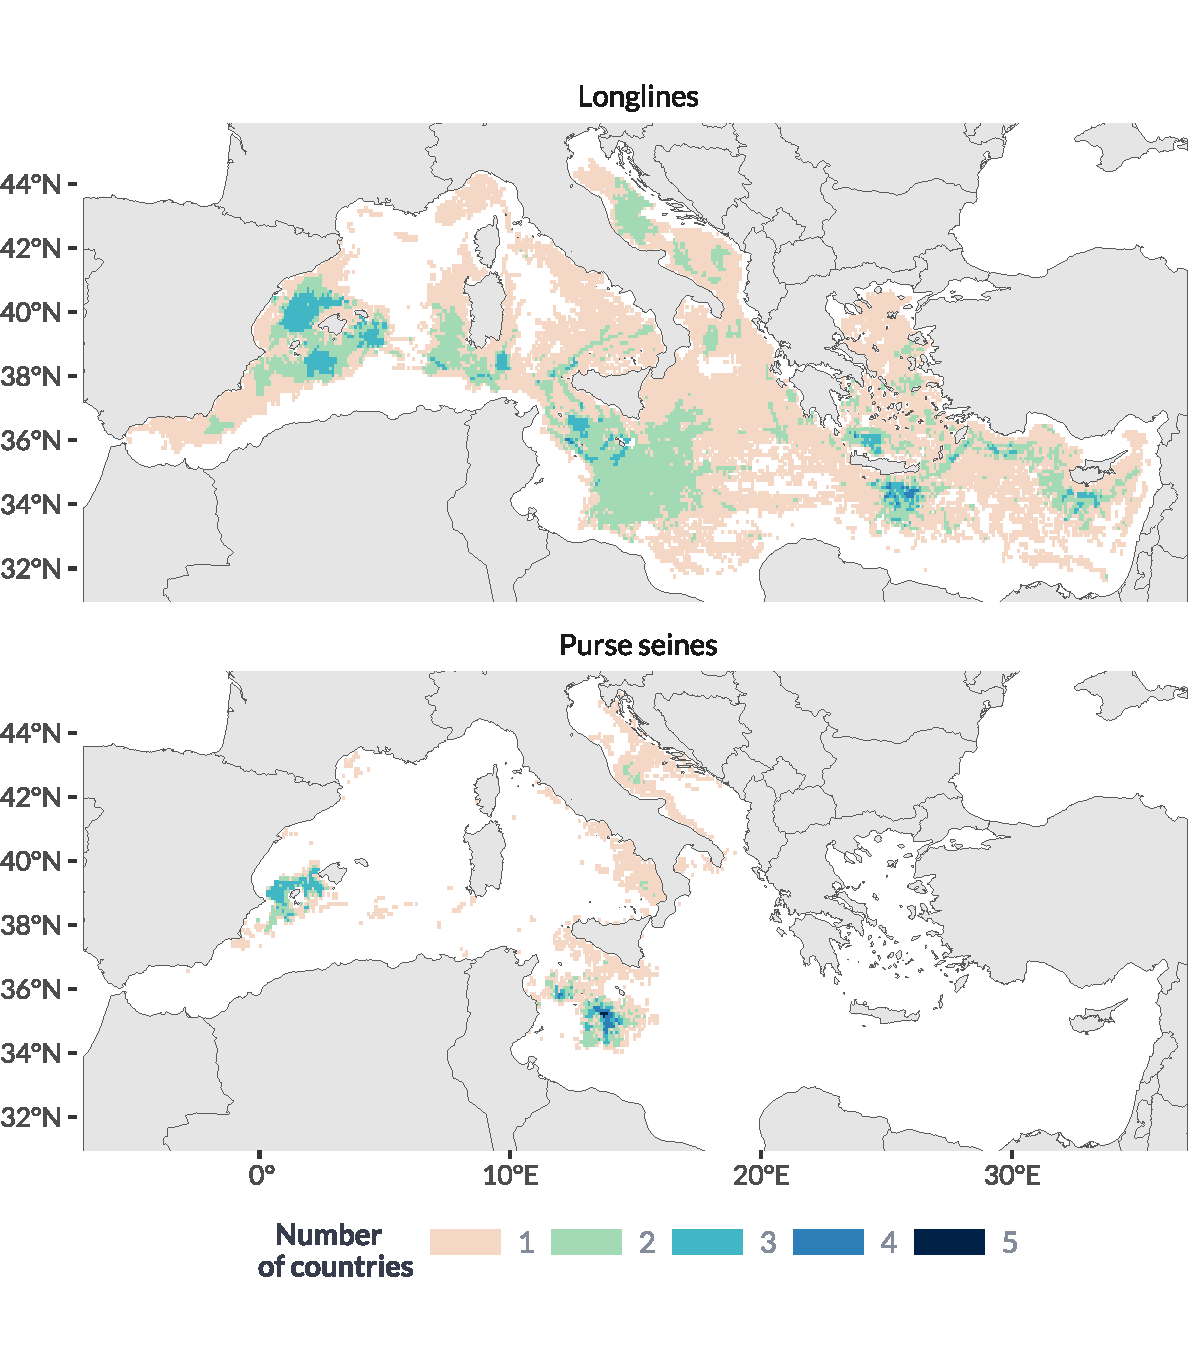
\includegraphics[width=1\linewidth, trim=0 1.2cm 0 1.2cm,clip]{Figures/plots/no_countries.pdf}
    \caption{Number of countries fishing per cell for longliners and purse seiners between 2015-2024.}
    \label{fig:no_countries}
\end{figure}

A comparison of fishing hours from the GFW data with catch data from ICCAT shows that AIS underrepresents fishing activity by non-EU countries relative to EU countries
\figref{fig:ais_iccat}. Even though, many non-EU countries account for a substantial share of the total reported catches. Notably, AIS also does not capture any French
longline vessels.

\begin{figure}[h]
    \centering
    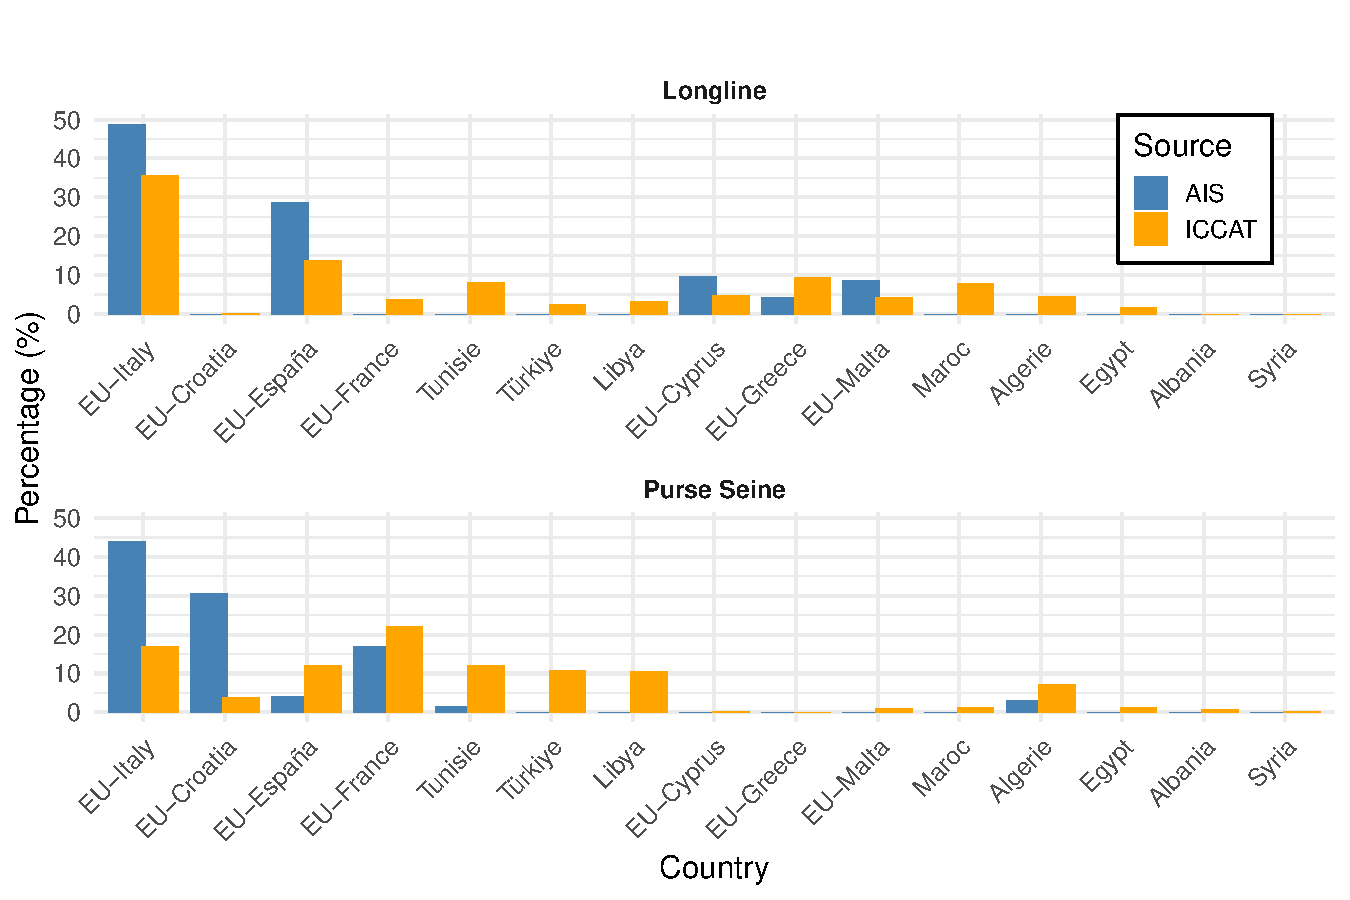
\includegraphics[width=1\linewidth, trim=0 0 0 1cm,clip]{Figures/plots/ais_vs_iccat.pdf}
    \caption{Comparison of relative percentages between GFW AIS data and ICCAT catch data. AIS percentages are relative to the
    total fishing hours between all countries. ICCAT percentages are relative to the total weight of catches between all countries.}
    \label{fig:ais_iccat}
\end{figure}

\FloatBarrier
\section{Depth and distance to port}

The relationship between the cumulative proportion of fishing hours and the distance to port reveals that most fishing activity of both gear types is concentrated
less than 100 km from the closest port \figref{sub0:fig:depth_dist}. The trend for the depth is different between gear types, where most purse seine
fishing occurs at shallower depths (below 1000 m) and longline effort takes place over much greater depth ranges \figref{sub1:fig:depth_dist}.

\begin{figure}[h]
    \customsubplot{2}
    {1\linewidth}                           % width
    {0 0 0 0}                       % trim
    {Figures/plots/depth_dist_both.pdf} % file
    {12,67}                                  % (A) position
    {58,67}                                  % (B) position
    {fig:depth_dist}
    {%
    Cumulative proportion of fishing hours with \subref{sub0:fig:depth_dist}) Distance to port and \subref{sub1:fig:depth_dist}) Depth.}
\end{figure}
